\section{Prediction of cell organelles}
\begin{figure}[htb]
    \centering
    \begin{minipage}{.5\textwidth}
      \centering
      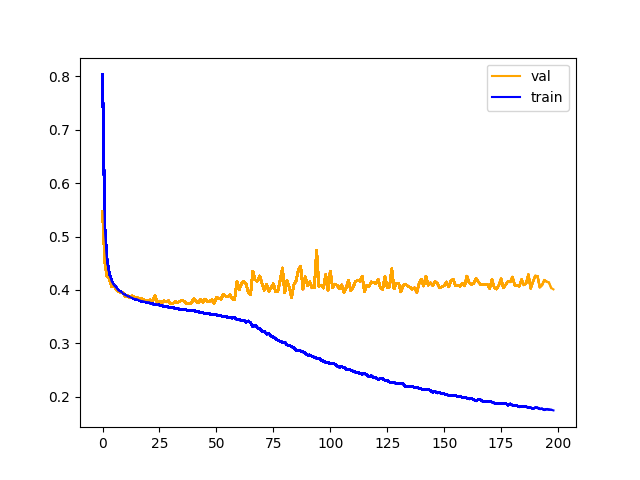
\includegraphics[width=\linewidth]{bilder/firt-train-overfit.png}
      \caption{Not regularized}
      \label{fig:first-train-overfit}
    \end{minipage}%
    \begin{minipage}{.5\textwidth}
      \centering
      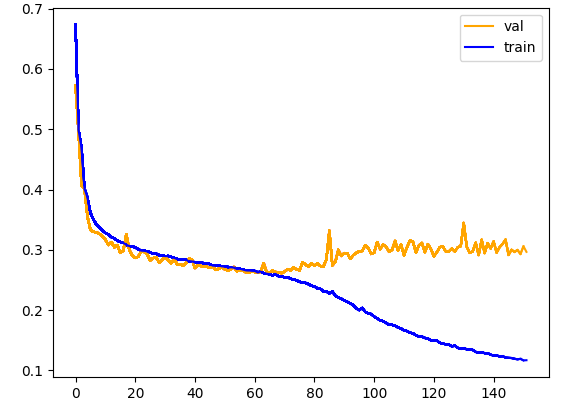
\includegraphics[width=\linewidth]{bilder/first-train-regularized.png}
      \caption{Regularized}
      \label{fig:first-train-regularized}
    \end{minipage}
\end{figure}

\subsection{Overfitting}

\begin{definition}[Overfitting]
    "Hypothesis overfits the training samples if some other hypothesis that fits the training samples less well actually performs better over the entire distribution of instances" (p67 Mitchell Machine Learning 1997).
\end{definition}

Overfiting prevents model to generalize well on the unseen data and in order to avoid fitting to closely to the training dataset one has several options:

Regulatize the model. This could be done either by reducing the number of the parameters, therefore by changing the model archticture. Or by adding regularization layers like BatchNorm or Dropout. Regularization can also be done by putting more resctritions on weights by adding their $L1$ or $L2$ norms to the loss function.

From the first training one can clearly see an overfit happening around epoch 30. Although one could use early-stopping and chose any epoch before overfit has happened, the better solution would be to regularize a network better. Therefore the $BatchNormalization$ layers have been added after the first Convolution laye in each ConvBlock and $TransposedConvBlock$. The results of training the regularized network is presented in Figure \ref{fig:first-train-regularized}.